\documentclass[border=5mm]{standalone}
\usepackage{tikz}

\begin{document}

\resizebox{12cm}{12cm}{%
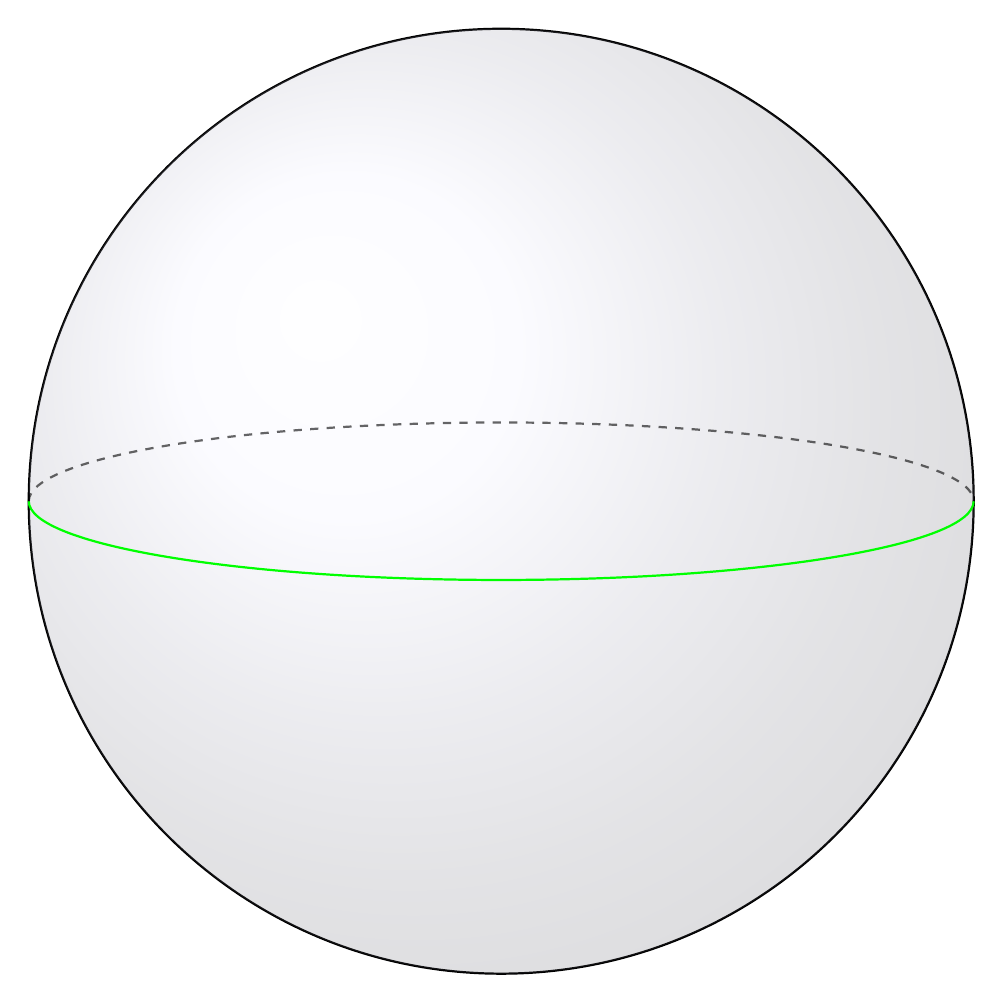
\begin{tikzpicture}

    % CELESTIAL SPHERE
    \draw[thick] (0,0) circle (6cm);
    \shade[ball color=blue!10!white, opacity=0.20] (0,0) circle (6cm);

    %\fill[fill=black] (0,0) circle (1pt);
    %\draw[dashed] (0,0 ) -- node[above]{$r$} (2,0);

    % EQUATOR
    \draw[thick, color=green] (-6,0) arc (180:360:6cm and 1cm);
    \draw[thick, dashed, opacity=.6] (-6,0) arc (180:0:6cm and 1cm);

    % EARTH
    %\draw[thick] (0,0) circle (0.5cm);
    %\shade[ball color=blue!60!white,opacity=0.80] (0,0) circle (0.5cm);

    % SUN
    %\draw[thick] (5.5024,2.392) circle (0.5cm);
    %\shade[ball color=yellow!60!white,opacity=0.8] (5.5024,2.392) circle (0.5cm);

    % ECLIPTIC OF THE SUN (front)
    %\draw[thick, rotate=23.5, color=blue] (-6,0) arc (180:360:6cm and 1cm);

    % ECLIPTIC OF THE SUN (bask)
    %\draw[thick, dashed, rotate=23.5, color=blue, opacity=.6] (-6,0) arc (180:0:6cm and 1cm);

    % VERNAL EQUINOX
    %\node[fill = black, draw = black, small dot = {right: }] at (0.2,-1) {};

    % DECLINATION ARROW
    %\draw[red, very thick, ->] (.2,-1) arc (-90:0:5.8 and 1.02);

    % RIGHT ASCENSION ARROW
    %\draw[green, very thick, ->] ++(6cm,0) arc (0:23:6cm);

\end{tikzpicture}
}

\end{document}